\section{Article du Monde du 3 mai 2015}
\tikzstyle{every picture}+=[remember picture]
\begin{frame}
	\frametitle{Le Monde -- 3 mai 2015 -- page 7}
	\centering
	\begin{tikzpicture}
		\node[inner sep=0pt] at (0,0) {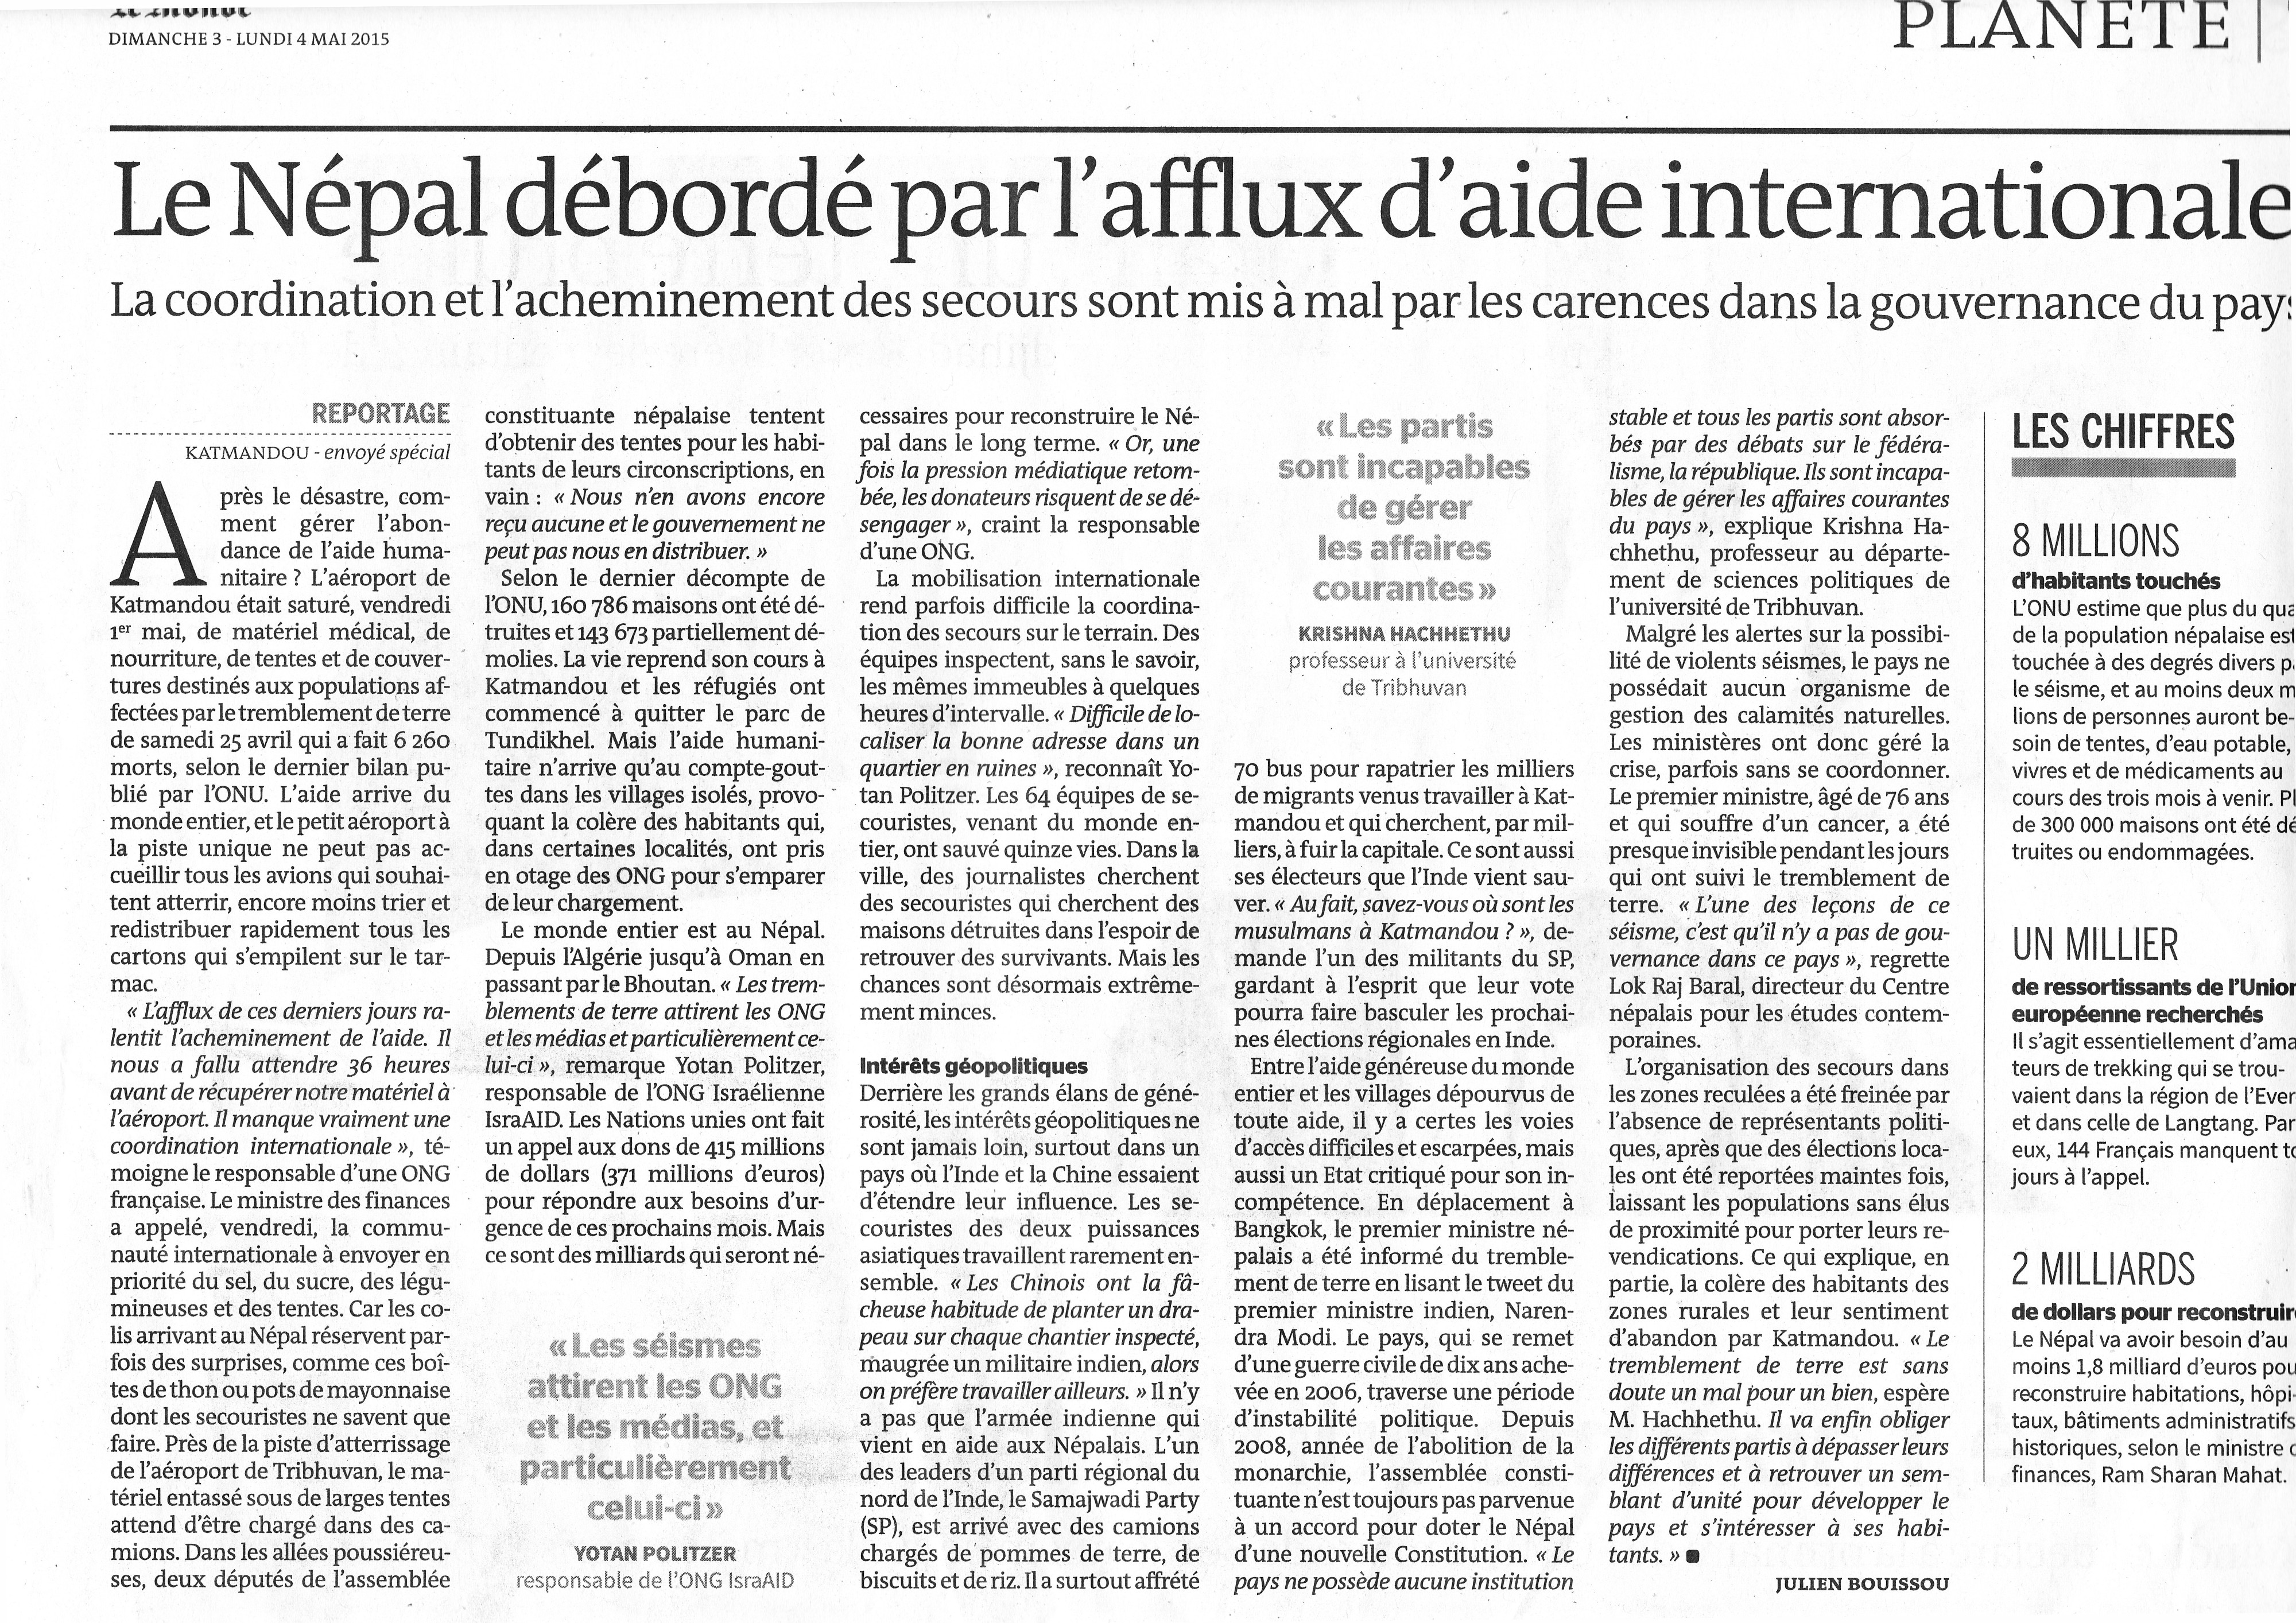
\includegraphics[height=8cm]{le_monde_small}};
		\onslide<2->{
			\draw[OrangeRed,ultra thick,rounded corners] (-5.3cm,3.5cm) rectangle (5.75cm,2.7cm);
		}
		\onslide<3->{
			\draw[LimeGreen,ultra thick,rounded corners] (-5.3cm,2.7cm) rectangle (5.75cm,2.3cm);
		}
		\onslide<4->{
			\draw[Orange,ultra thick,rounded corners] (-5.3cm,2.1cm) -- (0.35cm,2.1cm) -- (0.35cm,-1.1cm) -- (-1.55cm,-1.1cm) -- (-1.55cm,-4cm) -- (-5.3cm,-4cm) -- cycle;
			\draw[Orange,ultra thick,rounded corners] (4.1cm,2.1cm) -- (0.4cm,2.1cm) -- (0.4cm,-1.15cm) -- (-1.5cm,-1.15cm) -- (-1.5cm,-4cm) -- (4.1cm,-4cm) -- cycle;		
		}
		\onslide<5->{
			\draw[RoyalBlue,ultra thick,rounded corners] (0.5cm,2.025cm) rectangle (2cm,0.5cm);
			\draw[RoyalBlue,ultra thick,rounded corners] (-3.2cm,-2.45cm) rectangle (-1.65cm,-3.9cm);
		}
		\onslide<6->{
			\draw[Purple,ultra thick,rounded corners] (4.15cm,2.1cm) rectangle (5.75cm,-4cm) -- cycle;
		}
	\end{tikzpicture}
\end{frame}
\begin{frame}
	\frametitle{Le Monde -- 3 mai 2015 -- page 7}
	\begin{block}{Enjeux}
		\begin{itemize}
			\item Attirer le regard,
			\item Donner les grandes lignes au lecteur pressé,
			\item Présenter une situation très médiatique sans répéter trop de données,
			\item Donner des pistes de réflexion au lecteur attentif.
		\end{itemize}		
	\end{block}
\end{frame}

